\documentclass{article}
\title{Blanchard Ch.14}
\author{Dawei Wang}
\date{\today}
\usepackage{ctex}
\usepackage{amsmath}
\usepackage{amssymb}
\usepackage{graphicx} %插入图片的宏包
\usepackage{float} %设置图片浮动位置的宏包
\usepackage{subfigure} %插入多图时用子图显示的宏包
\begin{document}
	\maketitle	
\section{预期贴现值}

预期贴现值(expected present discounted value):一系列未来收益在今天的期望值。

\section{计算贴现值}

折现因子(discount factor):$ 1/(1+i_t) $。折现率$ i_t $。

预期贴现值(贴现值/现值):

\[
\$V_t=\$z_t+\frac{1}{1+i_t}\$z_{t+1}^e+\frac{1}{(1+i_t)(1+i_{t+1}^e)}\$z_{t+2}^e+\cdots
\]

固定利率和收益

\[
\$V_t=\$z_t[1+\frac{1}{(1+i)}+\cdots+\frac{1}{)(1+i)^{n-1}}]
\]

\[
\$V_t=\$z\frac{1-[1/(1+i)^n]}{1-1/[1+i]}
\]

固定利率和收益,无限期支付

\[
\$V_t=\frac{1}{(1+i)}\$z+\frac{1}{(1+i)^2}\$z+\cdots
\]

\[
\$V_t=\frac{\$z}{i}
\]

\hspace*{\fill}

名义利率、实际利率和现值

假设我们想要计算的是实际收益序列的现值,即以一揽子商品表示的收益,而非以美元表示的,则应使用实际利率:

\[
V_t=\$z_t+\frac{1}{1+r_t}\$z_{t+1}^e+\frac{1}{(1+r_t)(1+r_{t+1}^e)}\$z_{t+2}^e+\cdots
\]

这与用名义利率表示的现值是等价的,二者可以通过价格水平相联系起来:

\[
\frac{\$V_t}{P_t}=V_t
\]

我们可以通过两种方式计算一个收益序列的现值。一种是以美元表示的收益序列现值,使用名义利率折现,然后除以当前的价格水平。另一种是一揽子商品表示的收益序列现值,使用实际利率折现。

\section{债券价格和收益曲线}

债券之间的区别重要体现在以下两个方面。

期限(maturity)、风险。

不同期限的债券有各自的价格和相应的利率,称作到期收益率(yield to maturity),或简称为收益率(yield)。期限为一年甚至更短的债券的收益率称为短期利率(short-term interest rate)。更长期限的债券的收益率称为长期利率(long-term interest rate)。收益率和期限之间的关系称作收益率曲线(yield curve),或利率期限结构(term structure)

\hspace*{\fill}

债券分类:

政府债券:由政府或政府机构发行;

公司债券:由公司发行。

承诺在到期日一次性支付的债券称作贴现债券(discount bonds),一次性支付的额度称作债券的票面价值(face value)。

承诺在到期日前多次支付,并在到期日一次支付的债券称作息票债券(coupon bonds)。到期日前的支付叫作息票支付,最后一次支付称作债券的票面价值。

息票支付与票面价值的比值称作息票率(coupon rate)。当前收益率(current yield)是息票支付额和债券价格的比值。

从经济学的角度看,债券中对利率的正确测度是到期收益率。

美国联邦政府发行的发行时间不足一年的债券称作短期国库券(Treasury bills, T-bills)。它们是贴现债券,因此只在到期时一次性支付。发行时间为1~10年的债券称作中期国库券(Treasury notes)。发行时间期限为10年及十年以上的债券称作长期国库券(Treasury bonds)。中期债券和长期债券统称为息票债券。期限越长的债券风险越大,因此会享有一个风险溢价,也叫做期限溢价(term premium)。

债券通常是名义债券,它们承诺支付一系列固定的名义收益,该收益用本国货币计价。然而还有许多其他类型的债券。一种是指数化债券(indexed bonds),该债券承诺的收益是经过通货膨胀率调整的,而非固定的名义收益。


\hspace*{\fill}

债券评级:

债券评级越高,风险溢价越低,违约风险很高的债券有时被称作垃圾债券。

\subsection{作为现值的债券价格}

假设一年期债券承诺在明年支付100美元,价格记作$ P_{1t} $美元,令当前的一年期名义利率为$ i_{1t} $。

\[
\$P_{1t}=\frac{\$100}{1+i_{1t}}
\]

设两年期的债券承诺在两年后支付100美元,其价格记作$ P_{2t} $美元,且必然等于两年后100美元的现值,$ i^e_{1t+1} $:

\[
\$P_{2t}=\frac{\$100}{(1+i_{1t})(1+i^e_{1t+1})}
\]


\subsection{套利和债券价格}

假设持有一年期债券,对于投入的每一美元,明年都将得到$ (1+i_{1t}) $美元。

假设持有两年期债券,由于该债券的价格是$ P_{2t} $美元,对于现在投入的每一美元,第二年的预期得到$ \frac{P^e_{1t+1}}{P_{2t}} $。

假设投资者仅关心预期收益率,不关心持有二年期债券相较于一年期债券的风险,则由于套利者的存在,两种债券应该提供相同的一年期收益:

\[
1+i_{1t}=\frac{\$P^e_{1t+1}}{\$P_{2t}}
\]

即:

\[
\$P_{2t}=\frac{\$P^e_{1t+1}}{1+i_{1t}}
\]

$ \$P^e_{1t+1} $在明年的预期价格决定:

\[
\$P^e_{1t+1}=\frac{\$100}{1+i^e_{1t+1}}
\]

故:

\[
\$P_{2t}=\frac{\$100}{(1+i_{1t})(1+i^e_{1t+1})}
\]

套利的狭义条件:无法找到可以利用的无风险的收益机会。

\subsection{YTM(yield to maturity)}

YTM定义:一个n年期债券的YTM/n年期利率(n-year interest rate)为使今天的债券价格等于债券未来收益的现值的固定年利率。

两年期债券:

\[
\$P_{2t}=\frac{\$100}{(1+i_{2t})^2}
\]

\[
\frac{\$100}{(1+i_{2t})^2}=\frac{\$100}{(1+i_{1t})(1+i^e_{1t+1})}
\]

即:

\[
(1+i_{2t})^2=(1+i_{1t})(1+i^e_{1t+1})
\]

近似:

\[
i_{2t}\approx \frac{1}{2}(i_{1t}+i^e_{1t+1})
\]

长期利率反映了当前利率以及未来的预期短期利率。

\subsection{风险}

若投资者在持有两年期债券时希望获得一个风险溢价,则套利等式为:

\[
1+i_{1t}+x=\frac{\$P^e_{1t+1}}{\$P_{2t}}
\]

当一年期债券有一个已知的收益,即无风险时:

\[
\$P_{2t}=\frac{\$100}{(1+i_{1t})(1+i^e_{1t+1}+x)}
\]

计算YTM:

\[
\frac{\$100}{(1+i_{2t})^2}=\frac{\$100}{(1+i_{1t})(1+i^e_{1t+1}+x)}
\]

即:

\[
(1+i_{2t})^2=(1+i_{1t})(1+i^e_{1t+1}+x)
\]

近似:

\[
i_{2t}\approx 1/2(i_{1t}+i^e_{1t+1}+x)
\]

两年期利率是当前利率、未来一年期期望利率和风险溢价的平均值。假定下一年的一年期期望利率和今年一样,那么两年期利率将会高于一年期利率。因为价格风险会随着债券期限增加而增加,风险溢价也会随着期限的增加而增加,这说明收益率曲线一般会上扬,从而反映持有债券时间越长所承担风险越大这一情况。

\subsection{收益率曲线的解释}

当投资者利率是恒定的,收益率曲线应当略微上扬,反映了风险溢价随着期限增加。因此,当收益率曲线向下倾斜这一相对少见的情况出现时,说明投资者预期利率逐渐下降(为了保持经济增长,央行应当逐渐下调政策利率)。

\section{股票市场和股票价格的变动}

公司的四种筹集资金的方式:

1. 内部融资(internal finance),使用一部分利润;

2. 外部融资(external finance),银行贷款;

3. 债务融资(debt finance),即债券和贷款;

4. 股权融资(equity finance),发行股票。


\subsection{股票价格和现值}

股价必定等于未来预期红利的现值。

假定持有一年期股票,令$ \$Q_t $表示今年股价,$ \$D_t $表示今年的红利,$ \$D^e_{t+1} $表示明年的预期红利。假设今年的股价为除息价格。对于每一股,明年预期得到:$ (\$D^e_{t+1}+\$Q^e_{t+1}) $,对于购买股票的每一美元,预期得到:$ \frac{(\$D^e_{t+1}+\$Q^e_{t+1})}{\$Q_t} $。

相较于持有债券而言,持有股票更具风险,在股票中,风险溢价被称为股权溢价(equity premium)。则均衡要求持有股票一年收益率等于持有一年债券的收益率和股权溢价之和:

\[
\frac{(\$D^e_{t+1}+\$Q^e_{t+1})}{\$Q_t}=1+i_{1t}+x
\]

即:

\[
\$Q_t=\frac{\$D^e_{t+1}}{(1+i_{t1}+x)}+\frac{\$Q^e_{t+1}}{(1+i_{1t}+x)}
\]

\[
\$Q^e_{t+1}=\frac{\$D^e_{t+2}}{(1+i^e_{1t+1}+x)}+\frac{\$Q^e_{t+2}}{(1+i^e_{t+1}+x)}
\]

实际股价:

\[
Q_t=\frac{D^e_{t+1}}{1+r_{1t}+x}+\frac{D^e_{t+2}}{(1+r_{1t}+x)(1+r^e_{1t+1}+x)}+\cdots
\]

三层含义:

更高的预期未来实际红利带来更高的实际股票价格。

更高的当前和预期未来的一年期实际利率带来更低的股票价格。

更高的股权溢价带来更低的股票价格。

\subsection{股票市场和经济活动}

股票市场的变动很大程度上源自于不可预测性。股票价格遵从随机游走假说,股票变化的不可预测性是股票市场完善的标志。

假设预期通货膨胀率为零,因此,实际利率和名义利率相等。

\subsection{货币扩张和股票市场}

假设经济处于衰退阶段,美联储决定采取更加宽松的货币政策。货币的增加会导致LM曲线向下移动。

此时股票市场的反应取决于股票市场的参与者对货币政策的预期。如果他们已经完全预期到了扩张性货币政策,那么股票市场不会做出反应:不管是对未来红利的预期还是对未来利率的预期,已经被预期到的变动都不会产生影响,因此股价保持不变。

\begin{figure}[H] %H为当前位置,!htb为忽略美学标准,htbp为浮动图形
	\centering %图片居中
	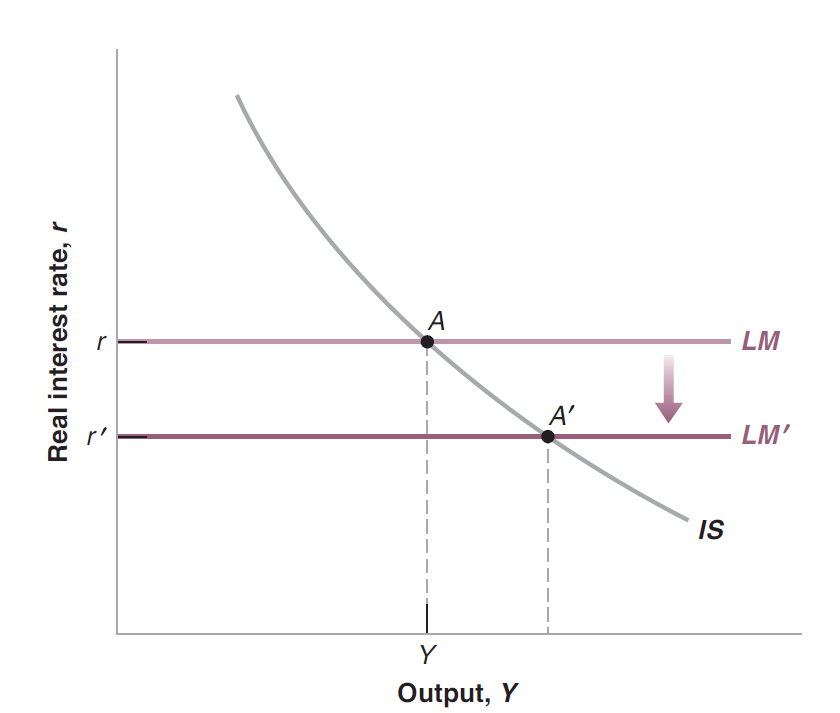
\includegraphics[width=1\textwidth]{14_1} %插入图片,[]中设置图片大小,{}中是图片文件名
	\caption{An Expansionary
		Monetary Policy and the
		Stock Market} %最终文档中希望显示的图片标题
	\label{Fig.main2} %用于文内引用的标签
\end{figure}

相反,假设美联储的举措至少部分未被预期到。在这种情况下,股价会上涨。原因有二:

1. 扩张性货币政策意味着一段时间内利率降低;

2. 这也意味着一段时间内产出提高,从而红利也会提高。

\subsection{消费支出的提高和股票市场}

考虑一个未被预测到的IS曲线右移情况,股价的变动取决于美联储的反应:

\begin{figure}[H] %H为当前位置,!htb为忽略美学标准,htbp为浮动图形
	\centering %图片居中
	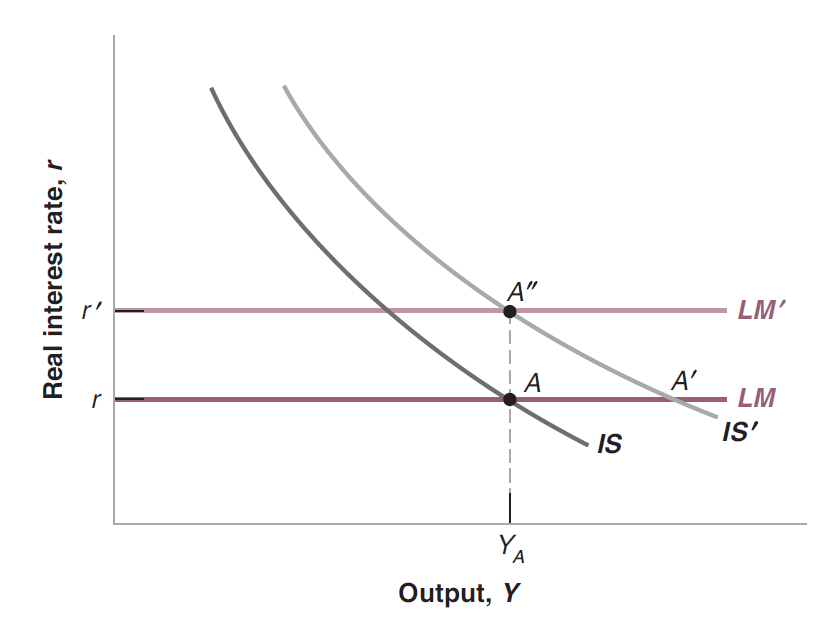
\includegraphics[width=1\textwidth]{14_2} %插入图片,[]中设置图片大小,{}中是图片文件名
	\caption{An Increase in
		Consumption Spending
		and the Stock Market} %最终文档中希望显示的图片标题
	\label{Fig.main3} %用于文内引用的标签
\end{figure}

若市场预期美联储保持政策利率不变,则产出增加利率不变,股价上升;若人们预期美联储担心产出高于$ Y_A $而导致通货膨胀,美联储若未上调政策利率抵消IS曲线的右移,使LM曲线上移,从LM曲线变为LM'曲线,此时产出不变而利率上升,股价下跌。

股票价格很大程度上取决于当前和未来经济活动的变化,但是这并不意味着任何股价和产出的简单关系都是如此。股价如何对应产出的变化取决于:

1. 市场先前的预期是什么;

2. 产出变动的来源;

3. 市场预期中央银行会对产出变化做出怎样的反应。

\section{风险、泡沫、狂热和股票价格}

并不是所有资产价格变动都源自于未来红利或者利率的消息,原因有二:

1. 风险会随时间变动;

2. 价格会偏离其基础价值。

\subsection{股价和风险}

股权溢价不是恒定的,因此股价的变动不仅来自未来股利和利率的预期,还来自股权溢价的变化。

\subsection{资产价格、基础价值和泡沫}

股票价格并不总是等于基础价值(fundamental value)。

只要投资者预期股价会上涨,股价就会上涨。这种股票价格呈现的变动被称作理性投机泡沫(rational speculative bubbles)。

如果人们预期股票价格在未来会进一步上涨,那么他们就愿意为该股票支付高于基础价值的价格。

并不是所有偏离基础价值的变动都是源自金融市场的理性泡沫,许多金融投资者都是非理性的。



\end{document}